\begin{defn}[Solenoidas]
  TODO: ~ritė
\end{defn}

\section{Elektromagnetinės indukcijos reiškinys}

\begin{figure}[H]
  \begin{center}
    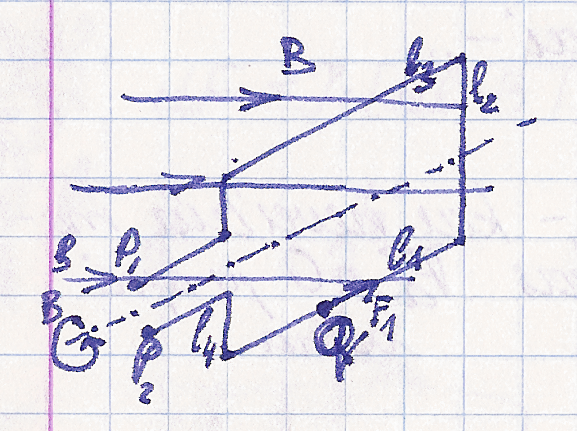
\includegraphics[height=0.5\textwidth]{images/remelis.png}
  \end{center}
  \caption{Rėmelis magnetiniame lauke}
  \label{fig:remelis}
\end{figure}

\begin{figure}[H]
  \begin{center}
    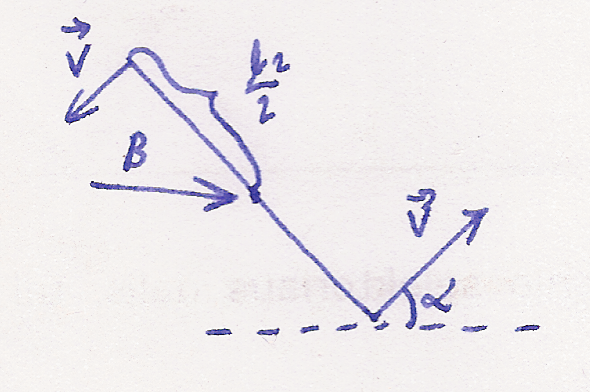
\includegraphics[height=0.5\textwidth]{images/besisukantis_laidininkas.png}
  \end{center}
  \caption{Besisukantis laidininkas}
  \label{fig:besisukantis_laidininkas}
\end{figure}

\begin{defn}[Indukcinė elektros srovė]
  Elektros srovė, kuri atsiranda laidininke, dėl magnetinio srauto
  kertančio to laidininko apribotą plotą, kitimo.
\end{defn}

Jeigu rėmelis sukasi magnetiniame lauke, tai tarp taškų $P_{1}$ ir
$P_{2}$ atsiranda potencialų skirtumas. Jėga veikianti krūvio nešėją,
kurio krūvis yra $q$, yra lygi:
\begin{align*}
  F_{1} =& q \cdot v \cdot B \cdot \sin \alpha \\
\end{align*}
čia:
\begin{description}
  \item[$v$] – laidininko dalies $l_{1}$ judėjimo greitis;
  \item[$B$] – magnetinė indukcija;
  \item[$\alpha$] – kampas tarp $\vec{B}$ ir $\vec{v}$.
\end{description}
Kadangi žinome, kad apskritimu judančio kūno greitis yra lygus to
kūno kampinio greičio ir apskritimo spindulio sandaugai, tai gauname:
\begin{align*}
  v &= \omega \frac{l_{2}}{2} \\
  F_{1} &= q \frac{\omega l_{2}}{2} B \sin \alpha \\
\end{align*}
Darbas, atliekamas perkeliant krūvį $q$, atkarpoje $l_{1}$ yra lygus:
\begin{align*}
  A_{1}
  &= F_{1} \cdot l_{1} \\
  &= q \frac{\omega l_{2}}{2} B \sin \alpha l_{1}, \\
  \intertext{o atkarpoje $l_{2}$ – $A_{2} = 0$, nes $\vec{F}$ ir $l_{2}$
  yra tarpusavyje statmeni. Iš viso, darbas atliekamas perkeliant krūvį
  iš taško $P_{1}$ į tašką $P_{2}$ yra lygus:}
  A
  &= A_{1} + A_{2} + A_{3} + A_{4} \\
  &= A_{1} + 0 + A_{3} + 0 \\
  &= 2 \cdot A_{1} \\
  &= q l_{2} l_{1} B \omega \sin \alpha \\
\end{align*}
Gauname, kad elektrovara laiko momentu $t$ yra lygi:
\begin{align*}
  \varepsilon
  &= \frac{A}{q} \\
  &= l_{2} l_{1} B \omega \sin \alpha \\
  &= S B \omega \sin \alpha \\
  &= B S \omega \sin \omega t \\
\end{align*}
Kadangi rėmelį veriantis magnetinis srautas yra lygus:
\begin{align*}
  \Phi_{B}
  &= \int B \cdot d S \\
  &= B l_{1} l_{2} \cos \alpha \\
  &= B S \cos \alpha \\
\end{align*}
tai gauname, kad:
\begin{align*}
  \frac{d \Phi_{B}}{d t}
  &= BS \cos \alpha |_{t} \\
  &= BS \cos \left( \omega t \right) |_{t} \\
  &= - \underbrace{BS \omega \sin \omega t}_{\varepsilon} \\
\end{align*}
Taigi:
\begin{align*}
  \varepsilon = -\frac{d \Phi_{B}}{d t} \\
\end{align*}

\begin{defn}[Faradėjaus elektromagnetinės indukcijos dėsnis]
  Jeigu $N$ vijų turintį, besisukantį kontūrą (žr.
  \ref{fig:remelis}) veria magnetinis laukas, tai tarp taškų $P_{1}$
  ir $P_{2}$ sukurta elektrovara yra lygi:
  \begin{align*}
    \varepsilon = - N \frac{d \Phi_{B}}{d t} \\
  \end{align*}
\end{defn}

\begin{defn}[Lenco taisyklė]
  Indukcijos elektrovaros kontūre sužadinta srovė visada teka tokia
  kryptimi, kad jos magnetinio lauko indukcija priešinasi pirminio
  magnetinio lauko kitimui.
\end{defn}

\begin{align*}
  F_{1} &=& q \cdot v \cdot B \cdot \sin \alpha \\
  v &=& w \cdot r \\
  F_{1} &=&  q \frac{w \cdot l_{2}}{2} B \sin \alpha \\
  A_{1} &=& F_{1} \cdot l_{1} \\
  &=& q \frac{w \cdot l_{2}}{2} \cdot l_{1} \cdot B \cdot \sin \alpha \\
  A_{2} &=& 0 \\
  A_{4} &=& 0 \\
  A_{3} &=& A_{1} \\
  A &=& A_{1} + A_{2} + A_{3} + A_{4} \\
  &=& 2 \cdot A_{1} \\
  &=& q \cdot l_{1} \cdot l_{2} \cdot B \cdot w \cdot \sin \alpha \\
  E &=& \frac{A}{q} \\
  &=& B \cdot S \cdot w \cdot \sin(wt) \\
  \Phi &=& \int B d S \\
  &=& B \cdot \underbrace{l_{1} \cdot l_{2}}_{S} \cdot \cos \alpha \\
  \frac{d \Phi}{d t} &=& -B \cdot S \cdot w \sin (wt) \\
  E &=& -\frac{d \Phi}{d t} &
    \t{Faradėjaus elektromagnetinės indukcijos dėsnis.} \\
  \Phi &=& B \cdot S \cdot \cos \alpha \\
  w &=& 2 \pi \nu \\
  &=& 2 \pi \frac{1}{T} \\
  e &=& \underbrace{B \cdot S \cdot w}_{E_{0}} \cdot \sin(wt) \\
  &=& E_{0} \sin(wt) \\
  i &=& I_{0} \sin(wt) \\
  X &=& \underbrace{X_{0}}_{A}
    \sin(\underbrace{wt + \varphi_{0}}_{\varphi}) \\
  I &=& \frac{U}{R} \\
\end{align*}
Čia:
\begin{description}
  \item[$E$] – elektrovara;
  \item[$A$] – darbas atliktas perkeliant krūvį $q$;
  \item[$w$] – kampinis greitis;
  \item[$\Phi$] – srautas; % FIXME Užbaigti.
  \item[$\nu$] – dažnis;
  \item[$T$] – periodas;
  \item[$e$] – momentinė elektrovara;
  \item[$i$] – momentinė srovė;
  \item[$A$] – svyravimo aplitudė;
  \item[$\varphi$] – svyravimo fazė;
  \item[$\varphi_{0}$] – svyravimo pradinė fazė;
\end{description}

\begin{defn}[Aplitudė]
  Didžiausia vertė, nuo pusiausvyros padėties.
\end{defn}

\begin{defn}[Kintamos srovės dažnis]
  Kiek kartų susvyravo per 1 sekundę.
\end{defn}

Efektinės įtampos ir srovės vertės.

\begin{align*}
  Q &=& I^{2} \cdot R \cdot t \\
  dQ &=& I^{2} \cdot R \cdot dt \\
  \int dQ &=&
    \int _{0} ^{T} I_{0}^{2} \cdot R 
    \cdot \sin^{2} \frac{2 \pi}{T} \cdot dt \\
  Q &=&  I^{2}_{0} R \frac{I}{2} \\
  I_{ef} &=&  \frac{I_{0}}{\sqrt{2}} \\
  E_{ef} &=&  \frac{E_{0}}{\sqrt{2}}
\end{align*}

\begin{exmp}
  % „L7106-4810TMP.pdf“
  Duota:
  \begin{align*}
    l &=& 0,6 m \\
    r_{0} &=& 0,2 m \\
    I &=& 30 A \\
  \end{align*}

  Bio-Savaro-Laplaso dėsnis:
  \begin{align*}
    dB &=& \frac{\mu_{0} \cdot l \cdot \sin \alpha}{4\pi r^2} dl \\
  \end{align*}
  
  \begin{align*}
    dl &=& \frac{r \cdot d \alpha}{\sin \alpha} \\
    r &=& \frac{r_{0}}{\sin \alpha} \\
    d B &=& \frac{\mu_{0} I \sin \alpha r d \alpha
      }{4 \pi r^2 \sin \alpha} \\
    &=& \frac{\mu_{0} I d \alpha}{4 \pi r} \\
    &=& \frac{\mu_{0} I}{4 \pi r_{0}} \sin \alpha d \alpha \\
  \end{align*}

  \begin{align*}
    B &=&
      2 \int _{0} ^{\arctan \frac{0,3}{0,2}}
      \frac{\mu_{0} I}{4 \pi r_{0}} \sin \alpha d \alpha \\
    &=& \frac{\mu_{0} I}{2 \pi r_{0}} \int _{0} ^{\arctan \frac{3}{2}}
      \sin \alpha d \alpha \\
    &=& \left. \frac{\mu_{0} I}{2 \pi r_{0}} \cos \alpha 
    \right| _{0} ^{\arctan \frac{3}{2}} \\
    &=& \frac{\mu_{0} I}{2 \pi r_{0}}
      \left( 1 - \cos\left( \arctan \frac{3}{2} \right) \right) \\
    \cos\left( \arctan \frac{3}{2} \right)
    &=& \frac{r_{0}}{\sqrt{\left(\frac{l}{2}\right)^{2} + r_{0}^{2}}} \\
    &=& \frac{0,2}{\sqrt{0,3^{2} + 0,2^{2}}} \\
    &=& 0,55470019622522915 \\ % FIXME Pakeisti lygybės ženklą.
    \mu_{0} &=& 4 \pi \cdot 10^{-7} \frac{H}{m} \\
    B &=& 2,496 \cdot 10^{-5} % Turėtų būti.
  \end{align*}
\end{exmp}
